\documentclass[11pt]{article}

\usepackage{times}
\usepackage{epsf}
\usepackage{epsfig}
\usepackage{amsmath, alltt, amssymb, xspace}
\usepackage{wrapfig}
\usepackage{fancyhdr}
\usepackage{url}
\usepackage{verbatim}
\usepackage{fancyvrb}

\usepackage{subfigure}
\usepackage{cite}
%\usepackage{cases}
%\usepackage{ltexpprt}
%\usepackage{verbatim}

%\topmargin      -0.70in  % distance to headers
%\headheight     0.2in   % height of header box
%\headsep        0.4in   % distance to top line
%\footskip       0.3in   % distance from bottom line

% Horizontal alignment
\topmargin      -0.50in  % distance to headers
\oddsidemargin  0.0in
\evensidemargin 0.0in
\textwidth      6.5in
\textheight     8.9in 


%\centerfigcaptionstrue

%\def\baselinestretch{0.95}


\newcommand\discuss[1]{\{\textbf{Discuss:} \textit{#1}\}}
%\newcommand\todo[1]{\vspace{0.1in}\{\textbf{Todo:} \textit{#1}\}\vspace{0.1in}}
\newtheorem{problem}{Problem}[section]
%\newtheorem{theorem}{Theorem}
%\newtheorem{fact}{Fact}
\newtheorem{define}{Definition}[section]
%\newtheorem{analysis}{Analysis}
\newcommand\vspacenoindent{\vspace{0.1in} \noindent}

%\newenvironment{proof}{\noindent {\bf Proof}.}{\hspace*{\fill}~\mbox{\rule[0pt]{1.3ex}{1.3ex}}}
%\newcommand\todo[1]{\vspace{0.1in}\{\textbf{Todo:} \textit{#1}\}\vspace{0.1in}}

%\newcommand\reducespace{\vspace{-0.1in}}
% reduce the space between lines
%\def\baselinestretch{0.95}

\newcommand{\fixmefn}[1]{ \footnote{\sf\ \ \fbox{FIXME} #1} }
\newcommand{\todo}[1]{
\vspace{0.1in}
\fbox{\parbox{6in}{TODO: #1}}
\vspace{0.1in}
}

\newcommand{\mybox}[1]{
\vspace{0.2in}
\noindent
\fbox{\parbox{6.5in}{#1}}
\vspace{0.1in}
}


\newcounter{question}
\setcounter{question}{1}

\newcommand{\myquestion} {{\vspace{0.1in} \noindent \bf Question \arabic{question}:} \addtocounter{question}{1} \,}

\newcommand{\myproblem} {{\noindent \bf Problem \arabic{question}:} \addtocounter{question}{1} \,}


\newcommand{\copyrightnoticeA}[1]{
\vspace{0.1in}
\fbox{\parbox{6in}{\small Copyright \copyright\ 2006 - 2014\ \ Wenliang Du, Syracuse University.\\ 
      The development of this document is partially funded by 
      the National Science Foundation's Course, Curriculum, and Laboratory 
      Improvement (CCLI) program under Award No. 0618680 and 0231122. 
      Permission is granted to copy, distribute and/or modify this document
      under the terms of the GNU Free Documentation License, Version 1.2
      or any later version published by the Free Software Foundation.
      A copy of the license can be found at http://www.gnu.org/licenses/fdl.html.}}
\vspace{0.1in}
}


\newcommand{\copyrightnotice}[1]{
\vspace{0.1in}
\fbox{\parbox{6in}{\small Copyright \copyright\ 2006 - 2014\ \ Wenliang Du, Syracuse University.\\
      The development of this document is/was funded by three grants from
      the US National Science Foundation: Awards No. 0231122 and 0618680 from
      TUES/CCLI and  Award No. 1017771 from Trustworthy Computing.
      This lab was imported into the Labtainer framework by the Naval Postgraduate 
      School, Center for Cybersecurity and Cyber Operations under National Science 
      Foundation Award No. 1438893.
      Permission is granted to copy, distribute and/or modify this document
      under the terms of the GNU Free Documentation License, Version 1.2
      or any later version published by the Free Software Foundation.
      A copy of the license can be found at http://www.gnu.org/licenses/fdl.html.}}
\vspace{0.1in}
}

\newcommand{\copyrightnoticeB}[1]{
\vspace{0.1in}
\fbox{\parbox{6in}{\small Copyright \copyright\ 2006 - 2014\ \ Wenliang Du, Syracuse University.\\
      The development of this document is/was funded by the following grants from
      the US National Science Foundation: No. 0231122, 0618680, and 1303306.
      Permission is granted to copy, distribute and/or modify this document
      under the terms of the GNU Free Documentation License, Version 1.2
      or any later version published by the Free Software Foundation.
      A copy of the license can be found at http://www.gnu.org/licenses/fdl.html.}}
\vspace{0.1in}
}


\newcommand{\nocopyrightnotice}[1]{
\vspace{0.1in}
\fbox{\parbox{6in}{\small  
      The development of this document is funded by 
      the National Science Foundation's Course, Curriculum, and Laboratory 
      Improvement (CCLI) program under Award No. 0618680 and 0231122. 
      Permission is granted to copy, distribute and/or modify this document.
      }}
\vspace{0.1in}
}

\newcommand{\idea}[1]{
\vspace{0.1in}
{\sf IDEA:\ \ \fbox{\parbox{5in}{#1}}}
\vspace{0.1in}
}

\newcommand{\questionblock}[1]{
\vspace{0.1in}
\fbox{\parbox{6in}{#1}}
\vspace{0.1in}
}


\newcommand{\minix}{{\tt Minix}\xspace}
\newcommand{\unix}{{\tt Unix}\xspace}
\newcommand{\linux}{{\tt Linux}\xspace}
\newcommand{\ubuntu}{{\tt Ubuntu}\xspace}
\newcommand{\selinux}{{\tt SELinux}\xspace}
\newcommand{\freebsd}{{\tt FreeBSD}\xspace}
\newcommand{\solaris}{{\tt Solaris}\xspace}
\newcommand{\windowsnt}{{\tt Windows NT}\xspace}
\newcommand{\setuid}{{\tt Set-UID}\xspace}
%\newcommand{\smx}{{\tt Smx}\xspace}
\newcommand{\smx}{{\tt Minix}\xspace}
\newcommand{\relay}{{\tt relay}\xspace}
\newcommand{\isys}{{\tt iSYS}\xspace}
\newcommand{\ilan}{{\tt iLAN}\xspace}
\newcommand{\iSYS}{{\tt iSYS}\xspace}
\newcommand{\iLAN}{{\tt iLAN}\xspace}
\newcommand{\iLANs}{{\tt iLAN}s\xspace}
\newcommand{\bochs}{{\tt Bochs}\xspace}

\newcommand\FF{{\mathcal{F}}}

\newcommand{\argmax}[1]{
\begin{minipage}[t]{1.25cm}\parskip-1ex\begin{center}
argmax
#1
\end{center}\end{minipage}
\;
}

\newcommand{\bm}{\boldmath}
\newcommand  {\bx}    {\mbox{\boldmath $x$}}
\newcommand  {\by}    {\mbox{\boldmath $y$}}
\newcommand  {\br}    {\mbox{\boldmath $r$}}


%\pagestyle{fancyplain}
%\lhead[\thepage]{\thesection}      % Note the different brackets!
%\rhead[\thesection]{SEED Laboratories}
%\lfoot[\fancyplain{}{}]{Syracuse University} 
%\cfoot[\fancyplain{}{}]{\thepage} 

\newcommand{\tstamp}{\today}   
%\lhead[\fancyplain{}{\thepage}]         {\fancyplain{}{\rightmark}}
%\chead[\fancyplain{}{}]                 {\fancyplain{}{}}
%\rhead[\fancyplain{}{\rightmark}]       {\fancyplain{}{\thepage}}
%\lfoot[\fancyplain{}{}]                 {\fancyplain{\tstamp}{\tstamp}}
%\cfoot[\fancyplain{\thepage}{}]         {\fancyplain{\thepage}{}}
%\rfoot[\fancyplain{\tstamp} {\tstamp}]  {\fancyplain{}{}}

\pagestyle{fancy}
%\lhead{\bfseries Computer Security Course Project}
\lhead{\bfseries SEED Labs}
\chead{}
\rhead{\small \thepage}
\lfoot{}
\cfoot{}
\rfoot{}

\usepackage{listings}
\usepackage{color}

\definecolor{dkgreen}{rgb}{0,0.6,0}
\definecolor{gray}{rgb}{0.5,0.5,0.5}
\definecolor{mauve}{rgb}{0.58,0,0.82}

\lstset{frame=tb,
  language=C,
  aboveskip=3mm,
  belowskip=3mm,
  showstringspaces=false,
  columns=flexible,
  basicstyle={\small\ttfamily},
  numbers=none,
  numberstyle=\tiny\color{gray},
  keywordstyle=\color{blue},
  commentstyle=\color{dkgreen},
  stringstyle=\color{mauve},
  breaklines=true,
  breakatwhitespace=true,
  tabsize=3
}




\lhead{\bfseries SEED Labs -- Web Tracking Lab}

\def \code#1 {\fbox{\scriptsize{\texttt{#1}}}}

\begin{document}

\begin{center}
{\LARGE Web Tracking Lab}
\end{center}

\copyrightnotice

\section{Lab Overview}
Behavioral targeting is a type of online advertising where ads are displayed based on the user’s web-browsing behavior. The user leaves a trail of digital foot prints moving from one website to the other. Behavioral targeting anonymously monitors and tracks the sites visited by a user. When a user surfs internet, the pages they visit, the searches they make, location of the user browsing from, device used for browsing and many other inputs are used by the tracking sites to collect data. A user profile is created from the data and data-mined for an online behavioral pattern of the user. As a result when users return to a specific site or a network of sites, the created user profiles are helpful in reaching the targeted audience to advertise. The targeted ads will fetch more user interest, the publisher (or seller) can charge a premium for these ads over random advertising or ads based on the context of a site.

\section{Lab Environment}

\newcommand{\urlorurls}{URLs }
\newcommand{\urlisorurlsare}{URLs are }

%%%%%%%%%%%%%%%%%%%%%%%%%%%%%%%%%%%%
%%% Part I of the environment setup
%\section{Lab Environment}

This lab runs in the Labtainer framework,
available at http://my.nps.edu/web/c3o/labtainers.
That site includes links to a pre-built virtual machine
that has Labtainers installed, however Labtainers can
be run on any Linux host that supports Docker containers.

From your labtainer-student directory start the lab using:
\begin{verbatim}
    start.py xsite
\end{verbatim}
Links to this lab manual and to an empty lab report will be displayed.  If you create your lab report on a separate system,
be sure to copy it back to the specified location on your Linux system.

\subsection{Environment Configuration}
This lab includes three networked computers as shown in 
Figure~\ref{fig:topology}. 
The "vuln-site" runs the Apache web server and the {\tt Elgg} web
applications.  The "attacker" and "victim" computers each include
the Firefox browser.  Use the browser {\tt Web Developer} / {\tt Network}
tool (upper right menu), to 
inspect the HTTP requests and responses.  

\begin{figure}[htb]
\begin{center}
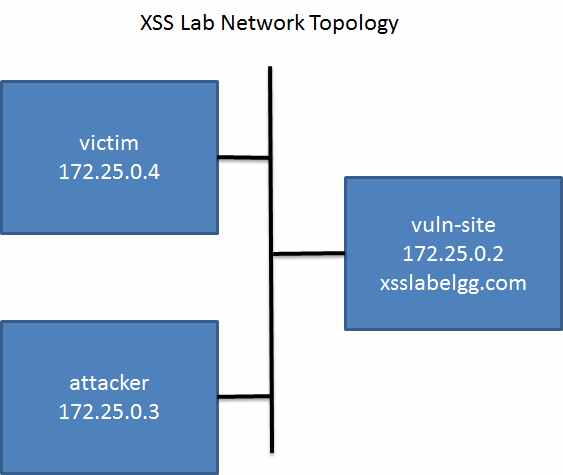
\includegraphics [width=0.8\textwidth,natwidth=621,natheight=403]{xsite.jpg}
\end{center}
\caption{Cross site scripting lab topology}
\label{fig:topology}
\end{figure}

\paragraph{Starting the Apache Server.}
The Apache web server will be running when the lab
commences.  If you need to restart the web server, use
the following command:
\begin{verbatim}
   % sudo systemctl restart httpd
\end{verbatim}

\paragraph{The {\tt Elgg} Web Application.}
We use an open-source web application called {\tt Elgg} in this lab.
{\tt Elgg} is a web-based social-networking application. 
It is already set up in on the vuln-site.
We have also created several user accounts on the {\tt Elgg} server and the credentials are given below.


\vspace{0.1in}
\begin{tabular}{|l|l|l|}
\hline
User 	& UserName 	& Password\\
\hline
Admin 	& admin 	& seedelgg \\
Alice 	& alice 	& seedalice \\
Boby 	& boby 		& seedboby \\
Charlie & charlie 	& seedcharlie \\
Samy 	& samy 		& seedsamy \\
\hline
\end{tabular}
\vspace{0.1in}


\paragraph{Configuring DNS.}
We have configured the following \urlorurls needed for this lab: 

%%%%%%%%%%%%%%%%%%%%%%%%%%%%%%%%%%%%


\vspace{0.1in}
\begin{tabular}{|l|l|l|}
\hline
URL & Description & Directory\\
\hline
\url{http://www.wtlabelgg.com } & Elgg web site & /var/www/webtracking/elgg \\
\url{http://www.wtcamerastore.com}  & CameraStore & /var/www/webtracking/CameraStore \\
\url{http://www.wtmobilestore.com }  & MobileStore & /var/www/webtracking/MobileStore \\
\url{http://www.wtelectronicsstore.com }  & ElectronicStore & /var/www/webtracking/ElectronicStore \\
\url{http://www.wtshoestore.com}  & ShoeStore & /var/www/webtracking/ShoeStore \\
\url{http://www.wtlabadserver.com }  & ReviveAdserver & /var/www/webtracking/adserver \\
\hline
\end{tabular}
\vspace{0.1in}



\subsection{Clear History and cookies} 

Please follow the instructions to {\tt clear history} and {\tt cookies} from the Firefox browser.

\begin{enumerate}
  \item Within the Firefox browser, select {\tt Preferences} per Figure ~\ref{fig:clear_history1} from the top-right menu button, and click on {\tt Privacy and Security} as shown in Figure ~\ref{fig:clear_history2} 
and then click the
{\tt Clear Recent History…} per ~\ref{fig:clear_history3}. A window {\tt Clear All History} pops up, as shown in Figure ~\ref{fig:clear_history4}

	\begin{figure}
	\centering	
	\begin{subfigure}
	\centering	
	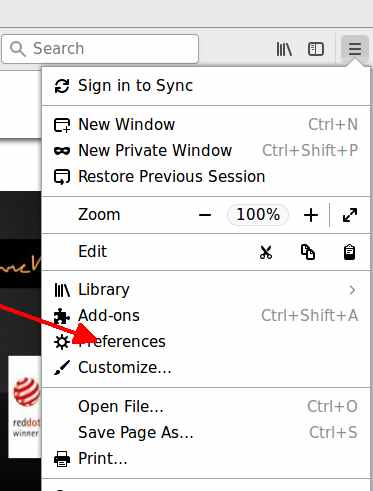
\includegraphics[width=0.4\textwidth,natwidth=621,natheight=403]{Figs/clearhistory1.jpg}
	\caption{select Preferences.} 
	\label{fig:clear_history1}
	\end{subfigure}%
	\begin{subfigure}
	\centering	
	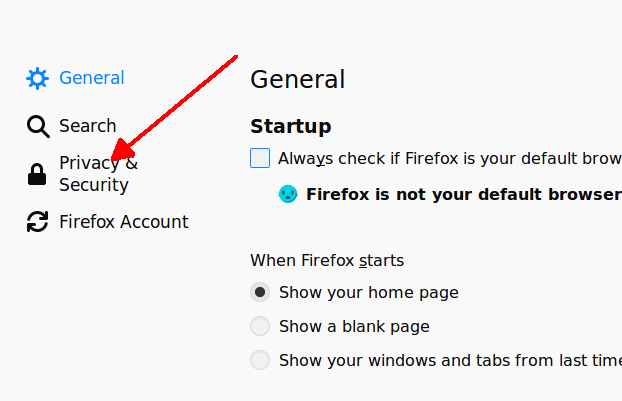
\includegraphics[width=0.4\textwidth,natwidth=621,natheight=403]{Figs/clearhistory2.jpg}
	\caption{Privacy and Security.} 
	\label{fig:clear_history2}
	\end{subfigure}
	\end{figure}
	\begin{figure}[ht]
	\centering	
	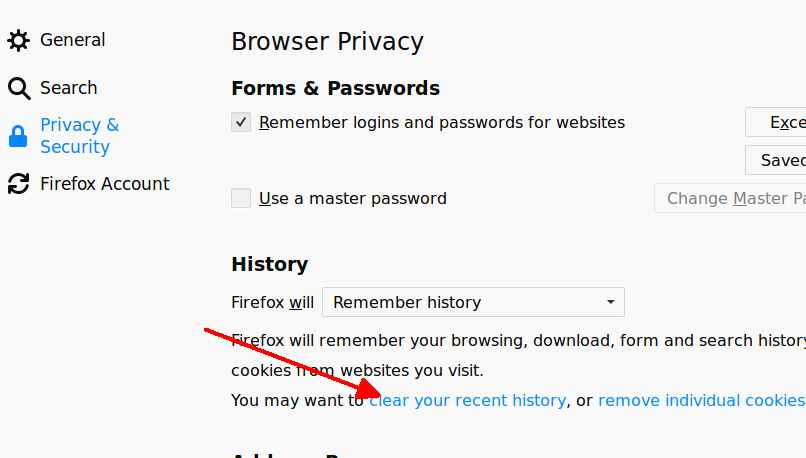
\includegraphics[width=0.4\textwidth,natwidth=621,natheight=403]{Figs/clearhistory3.jpg}
	\caption{Clear recent history.} 
	\label{fig:clear_history3}
	\end{figure}

  \item Select all the check boxes and Click on {\tt Clear Now} button in the pop up window. 
	\begin{figure}[ht]
	\centering	
	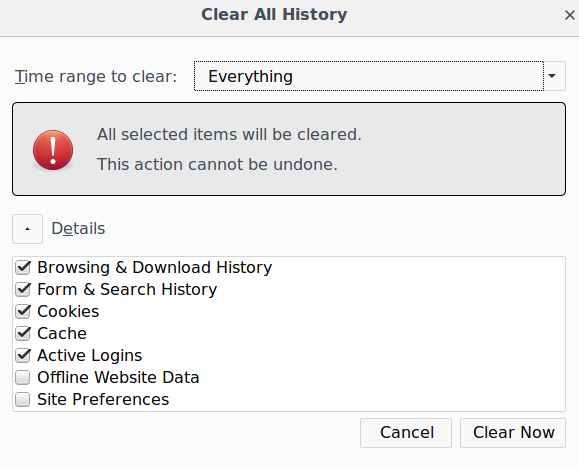
\includegraphics[width=0.4\textwidth,natwidth=621,natheight=403]{Figs/clearhistory4.jpg}
	\caption{Clear history and cookies.} 
	\label{fig:clear_history4}
	\end{figure}

\end{enumerate}
	

\subsection{Open a new private window in Firefox} 

Please follow the instructions to open a new private window in Firefox and start a private browsing session.

\begin{enumerate}
  \item With Firefox running, click on the menu button (upper-right) and welect {\tt Open a New Private Window} option as shown in Figure ~\ref{fig:private_window}

	\begin{figure}
	\centering	
	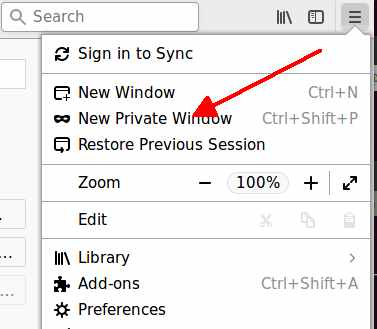
\includegraphics[width=0.4\textwidth,natwidth=621,natheight=403]{Figs/privatewindow.jpg}
	\caption{Open a private browser in Firefox.} 
	\label{fig:private_window}
	\end{figure}

  \item New Private browsing Firefox window opens up, start browsing in that private browser.


\end{enumerate}


\subsection{Note for Instructors} 

This lab may be conducted in a
supervised lab environment. The instructor may provide the following
background information to students at the beginning of the lab session:
\begin{enumerate}
  \item Information on how to use the pre-configured virtual machine.
  \item How to use Firefox and the Developer Storage Inspector and
the Firefox {\tt LiveHTTPHeaders} Extensions.
  \item A brief overview of the tasks.
       
\end{enumerate}


\section{Lab Tasks}


\subsection{Task 1: Understand the basic working of the web tracking}

Nowadays the online web user tracking helps in displaying ads to the targeted audience. 
When a user visits a website, there are certain ads, of which some of them are targeted advertisements. 
Say a user visits a certain product in an E-commerce website, he visits the product multiple times, checks the reviews and reads more about the product.
Sometime later when the user visits another website, to his surprise he finds the previously visited product is displayed as an advertisement.

The objective of this task is to understand the basic working of the web tracking. 
In this task you need to open the E-commerce websites, view details of one or more products. 
Once you login to the {\tt Elgg} website you should see the most visited product displayed as an advertisement. 


\begin{enumerate}
  \item Open {\tt Elgg} website without visiting any website and describe your observation in the lab report.
  \item Open Firefox and open the {\tt CameraStore}, {\tt MobileStore}, {\tt ElectronicStore} and {\tt ShoeStore} websites.
  \item Click on view details for any products in the websites.
  \item Refresh the {\tt Elgg} website in Firefox and describe your observation.
  \item Close the browser, reopen it and browse the {\tt Elgg} website. Describe your observation.       
\end{enumerate}


Note: If you want to repeat the observations for step 1, clear the {\tt Browsing History} and {\tt Cookies} from the Firefox browser.
Please follow the instructions to clear {\tt history} and {\tt cookies} in section 2.2

\subsection{Task 2: Importance of cookie in Web tracking}

{\tt Cookies} are created when a user's browser loads a particular website. The website sends information to the browser which then creates a text file. 
Every time the user goes back to the same website, the browser retrieves and sends this file to the website's web server. 
Computer {\tt Cookies} are created not just by the website that the user is browsing but also by other websites that run ads, widgets, or other elements on the web page which are being loaded. 
These {\tt cookies} regulate the ad display and functioning of other elements on the web page.

The objective of this task is to understand the importance of {\tt cookie} in web tracking. 
In this task you need to identify the tracking {\tt cookie} using the {\tt LiveHTTPHeaders} in Firefox. 
Please follow the steps below and give your observation.

\begin{enumerate}
  \item Open any one of the E Commerce websites {\tt CameraStore}, {\tt MobileStore}, {\tt ElectronicStore} and {\tt ShoeStore}.
  \item Click on view details for any product in websites and capture {\tt LiveHTTPHeader} traffic.
  \item In {\tt LiveHTTPHeaders}, identify the HTTP request, which set the {\tt third party cookies}, and take the screenshot.
  \item Right click on the productDetail page and select {\tt View Page Source}. Find out how the request for tracking {\tt cookie} is sent from the webpage, please take a screenshot and describe your observation.
\end{enumerate}

Third party {\tt cookies} are {\tt cookies} that are set by web site with a domain name other than the one the user is currently visiting. 
For example, user visits website abc.com, say the web page abc.com has an image to fetch from xyz.com. 
That image request can set {\tt cookie} on domain xyz.com, and the {\tt cookie} set on xyz.com domain is known as a {\tt third-party cookie}. 
Some advertisers use these types of {\tt cookies} to track your visits to the various websites on which they advertise.

The objective of this task is to understand how {\tt third party cookies} are used in web tracking. 
In this task you need to identify the third party {\tt cookie} using the Firefox Developer Storage Inspector, which can be viewed using
the upper-right menu, select ``Developer'' and then ``Storage Inspector''. 
Please strictly follow the steps below and record your observation.

\begin{enumerate}
  \item Open any one of the E Commerce websites {\tt CameraStore}, {\tt MobileStore}, {\tt ElectronicStore}, {\tt ShoeStore} and view details for any product.
  \item Open the ad server web page \url{ http://www.wtlabadserver.com}.
  \item Open the Storage Inspector on both pages and observe its displayed Cookie values. Switch between the products webpage and ad server webpage. 
	Describe your observation. (Please do NOT reload the products webpage).
\end{enumerate}

Identify the {\tt third party cookie} used for tracking in {\tt Storage Inspector}. 
Describe your observations in the report and explain why is it called a {\tt third party cookie}? 
Give reasons and screenshots to support your observation. 
A high-level architecture guideline is given in section 4, Figure~\ref{fig:guideline_figure}.

Note: If you wish to redo the task from beginning, please delete {\tt history} and {\tt cookies} from your Firefox browser. 
Please follow the instructions to {\tt clear history} and {\tt cookies} in section 2.2

\subsection{Task 3: Tracked user interests and data}


The ad servers update their database from users browsing history. 
They keep track of the web pages visited, articles read, videos watched and any other footprints which user can provide. 
The objective of this task is to figure out the user interests and view the logged user impressions. 
In this task you need to understand that all the products viewed by you will be logged in the ad server database. 
Please follow the steps below and give your observation.

\begin{enumerate}
  \item Open the E Commerce websites {\tt CameraStore}, {\tt MobileStore}, {\tt ElectronicStore} and {\tt ShoeStore}.
  \item Click on view details for any product in the website.
  \item Open \url{www.wtlabadserver.com/preferences.php} in a new tab and observe the webpage. 
\end{enumerate}

Explain how the user impressions are logged in ad server database, and how is it mapped to a user. 
Provide evidence to support your observation.

\subsection{Task 4: How ads are displayed in website}

The ad servers use the user profile (browsing history, recent product visits) to display the advertisements and now that the {\tt cookie} is set to track the user, 
the ad servers display the targeted advertisements. 

In this task you need to observe how the ad is rendered and displayed in the website. 
Please follow the steps below and give your observation.
\begin{enumerate}
  \item Open the {\tt Elgg} website in Firefox browser.
  \item Capture and observe the {\tt LiveHTTPHeader} traffic of the {\tt Elgg} website, identify the HTTP requests which are from a different {\tt domain} (third party).
\end{enumerate}

Explain in detail how the {\tt Elgg} website displays the targeted ads of the user. 
Provide evidence to support your explanation. 
(Hint: Use the table displayed in Task3 and {\tt LiveHTTPHeader} traffic in Task2).

\subsection{Task 5: Tracking in a Private browser window}


In {\tt InPrivate} browsing the browser stores some information such as {\tt cookies} and temporary Internet files so the webpages you visit will work correctly. 
However, at the end of your {\tt InPrivate} browsing session, this information is discarded. 
Once the {\tt InPrivate} browser is closed the {\tt cookies} are cleared, and temporary internet files are deleted for that session.

The objective of this task is to understand the working of the web tracking in a private browser window. 
In this task you need to open the E-commerce websites, view details of one or more products. 
Once you login to the {\tt Elgg} website (in the same private browser) you should see the most visited product displayed as an advertisement.

\begin{enumerate}
  \item Open {\tt Elgg} website without visiting any website and describe your observation in the lab report.
  \item Open Firefox and open the {\tt CameraStore}, {\tt MobileStore}, {\tt ElectronicStore} and {\tt ShoeStore} websites.
  \item Click on view details for any products in the websites.
  \item Refresh the {\tt Elgg} website in Firefox and describe your observation.
  \item Close the {\tt InPrivate} browser, reopen it and browse the {\tt Elgg} website. Describe your observation.
\end{enumerate}

Compare your observations with Task1. Explain the reasons and provide evidence to support your observations.

Note: Please follow the instructions in section 2.3 to open a new private window in Firefox.

\subsection{Task 6: Real world tracking}

The web tracking in real world involves many ad servers, each ad servers have their own technique of tracking the user interests. 
In this task you need to visit any of the websites given below and identify the web requests which are sent to the ad servers using the {\tt LiveHTTPHeaders} in Firefox.
The websites are:

\begin{enumerate}
  \item \url{http://dictionary.reference.com}
  \item \url{http://www.amazon.com}
  \item \url{http://www.careerbuilder.com}
\end{enumerate}

Open the websites, observe the HTTP request and response in {\tt LiveHTTPHeaders}. 
Capture screenshot of one HTTP request to the real world ad server for each web site. 
Also identify the {\tt third party cookie} used for that HTTP request.

\subsection{Task 7: Countermeasures}

There are certain countermeasures for the web tracking but most of the websites won’t work properly after implementing the counter measures. 
Most of the websites are highly dependent on {\tt JavaScript} and {\tt third party cookies}. 
You must have observed that the web tracking tasks are mostly dependent on the {\tt third party cookies}.

The objective of this task is to understand the countermeasures. 
In this task you should disable the {\tt third party cookies} in Firefox browser and figure out if your impressions are tracked. 
Please follow the steps below and give your observation:

\begin{enumerate}
  \item Disable the {\tt third party cookies} from the Firefox browser. Please follow the instructions of how to disable {\tt third party cookies} in Firefox browser in \url{https://support.mozilla.org/en-US/kb/disable-third-party-cookies}.
  \item After disabling the third party {\tt cookies}, open the {\tt CameraStore}, {\tt MobileStore}, {\tt ElectronicStore}, {\tt ShoeStore} websites and {\tt LiveHTTPHeaders}.
  \item Click on view details for any products in the websites.
  \item In {\tt LiveHTTPHeaders}, identify the HTTP request, which set the {\tt third party cookies}, and take the screenshot.
  \item Open {\tt Elgg} website and describe your observation. Also take the screenshot of HTTP request to ads server in {\tt LiveHTTPHeaders}. Compare it with the HTTP request to ads server in Task 4 and explain the difference.

\end{enumerate}

Also there are other ways to mitigate the web tracking. To opt out of targeted advertisement, 
add browser extensions like RequestPolicy, NoScript and Ghostery which control the third party requests from the web browser. 
Also one can keep {\tt cookies} for the browsing session, by setting a {\tt cookie} policy “only keep cookies until I close my browser” 
which will delete all the {\tt cookies} after the browser window is closed. 

Major web browsers provide with an option of {\tt Do Not Track}, which is a feature to let third party trackers know your preference to opt out third party tracking, 
and it is done by sending a HTTP header for every web request. 
This {\tt Do Not Track} preference may or may not adhered by the third party trackers. 
Some third party trackers provide with an option of {\tt Opt Out} of targeted advertisement. 
Some of them may interpret "Opt Out" to mean "do not show me targeted ads", rather than "do not track my behavior online". 
You can check your tracked online profile created by Google in \url{www.google.com/settings/ads}. 
You can also find the Opt out option provided in the above Google URL.

\section{Guidelines}

The diagram in Figure~\ref{fig:guideline_figure} shows the high level architecture of the Web tracking. 
In this diagram we have three major components, the {\tt E-Commerce} websites, {\tt Ad server} and the {\tt Elgg} website to display the targeted advertisements. 
Each of the e-commerce websites have {\tt web bugs} or {\tt beacons} to track user preferences. 
They are implanted as 1px by 1px image tags in the websites.

	\begin{figure}
	\centering
	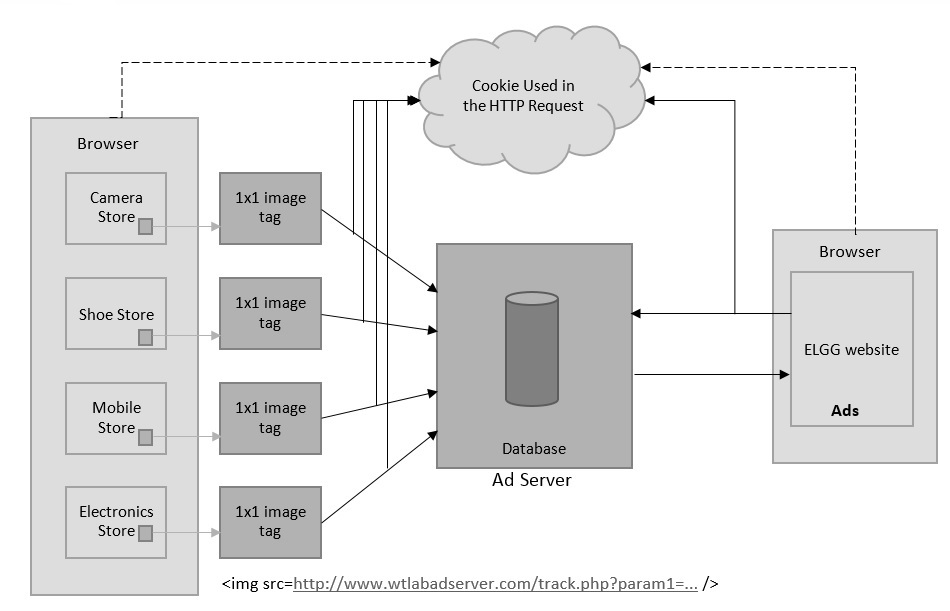
\includegraphics[width=0.8\textwidth,natwidth=621,natheight=403]{Figs/Guidelinefigure.jpg}
	\caption{High level architecture diagram of web tracking} 
	\label{fig:guideline_figure}
	\end{figure}


\section{Submission}

You need to submit a detailed lab report to describe what you have
done and what you have observed. Please provide details using 
{\tt LiveHTTPHeaders}, and/or screen shots. 
You also need to provide explanation
to the observations that are interesting or surprising.
If you edited your lab report on a separate system, copy it back to the Linux system at the location
identified when you started the lab, and do this before running the stop.py command.

After finishing the lab, go to the terminal on your Linux system that was used to start the lab and type:
\begin{verbatim}
./stop.py webtrack
\end{verbatim}
When you stop the lab, the system will display a path to the zipped lab results on your Linux system.  Provide that file to
your instructor, e.g., via the Sakai site.


\begin{thebibliography}{10}


\bibitem{httpcookieitem}
HTTP Cookie - Wikipedia. Available at the following URL:

\newblock \url{http://en.wikipedia.org/wiki/HTTP_cookie}.

\bibitem{newcookie}
New Cookie Technologies : Harder to See and Remove, Widely Used to Track you 


https://www.eff.org/deeplinks/2009/09/new-cookie-technologies-harder-see-and-remove-wide



\bibitem{onlinetracking}
How Online Tracking companies know most of what you do online

\newblock \url{https://www.eff.org/deeplinks/2009/09/online-trackers-and-social-networks}.


\end{thebibliography}


\end{document}

